\documentclass[conference]{IEEEtran}
\IEEEoverridecommandlockouts
\usepackage{cite}
\usepackage{amsmath,amssymb,amsfonts}
\usepackage{algorithmic}
\usepackage{graphicx}
\usepackage{textcomp}
\usepackage{xcolor}
\usepackage{url}
\def\BibTeX{{\rm B\kern-.05em{\sc i\kern-.025em b}\kern-.08em
    T\kern-.1667em\lower.7ex\hbox{E}\kern-.125emX}}

\begin{document}
\urlstyle{same}
\Urlmuskip=0mu plus 2mu

\title{Zero-Knowledge Private Zakat: A Privacy-Preserving Donation Protocol for Blockchain-Based Islamic Social Finance}

\author{
\IEEEauthorblockN{Muhammad Zidan Fatonie}
\IEEEauthorblockA{\textit{School of Computer Science}\\
\textit{BINUS University}\\
Jakarta, Indonesia\\
muhammad.fatonie@binus.ac.id}
}

\maketitle

\begin{abstract}
Zakat, one of the five pillars of Islam, represents a mandatory annual obligation for wealth redistribution with profound social welfare implications. Despite growing interest in blockchain-based zakat platforms, existing systems expose complete donor-recipient transaction records on public ledgers, creating a fundamental tension with Islamic principles of dignity preservation. This paper proposes a Zero-Knowledge Private Zakat (ZK-PZ) protocol that enables cryptographically private donations while maintaining verifiable transparency and Sharia compliance. The proposed architecture leverages Aztec Network's private transaction infrastructure, implementing programmable privacy through Noir smart contracts, nullifier-based double-donation prevention, and selective disclosure mechanisms. Donors can contribute zakat with complete anonymity or selective disclosure while recipients receive disbursements through encrypted private notes. The protocol preserves institutional trustworthiness through on-chain verification of proof validity while eliminating public exposure of individual transaction data. A prototype implementation on Ethereum Sepolia demonstrates technical feasibility, with UltraHONK proof generation averaging 262 ms and on-chain donation gas costs of approximately 490K gas per transaction. This work proposes a domain-specific privacy protocol designed for Islamic social finance, directly addressing the maqasid al-shariah imperative of nafs (dignity) protection.
\end{abstract}

\begin{IEEEkeywords}
Zero-Knowledge Proofs, Aztec Network, Noir, Blockchain, Zakat, Privacy-Preserving Donations, Islamic FinTech, Sharia Compliance, Nullifier Mechanism, Ethereum Sepolia
\end{IEEEkeywords}

\section{Introduction}

Zakat management at the intersection of Islamic jurisprudence and modern blockchain infrastructure presents both an opportunity and a challenge. BAZNAS [1] reports that the annual zakat potential in Indonesia alone is estimated at Rp~327 trillion (approximately USD~20 billion), while actual collection remains a fraction of that figure.

The advent of distributed ledger technology has prompted substantial research into blockchain-based zakat systems. Babas et al. [2] demonstrated that blockchain can provide decentralized zakat collection and distribution. Nazeri et al. [3] found that blockchain features such as transparency, traceability, and security align with zakat management objectives in Malaysia. Khairi et al. [4] developed a zakat collection blockchain system that offers automated disbursement and an immutable audit trail. However, these systems introduce a critical privacy paradox: by placing complete donor-recipient transaction records on public ledgers, they inadvertently expose socioeconomic vulnerabilities. The principle of maqasid al-shariah (objectives of Islamic law) explicitly protects \textit{nafs} (life and dignity) of individuals [5, 6]. In Islamic jurisprudence, preservation of donor and recipient privacy during charitable giving is considered a virtuous act that maintains dignity for both parties.

Zero-Knowledge Proofs (ZKPs) offer a cryptographic resolution to this paradox. Hameed et al. [7] survey ZKP constructions, and Wen et al. [8] analyze non-interactive variants (zk-SNARKs) suitable for blockchain deployment. The Aztec Network [9] provides an infrastructure for privacy-preserving transactions on Ethereum. Through its hybrid public-private state model, Aztec enables donors to transact with complete shielding: only the donor, recipient, and smart contract can decrypt transaction details. The network utilizes Noir circuits [10] for programmable privacy logic and the UltraHONK proof system for efficient verification. Despite these advances, no prior work has proposed a domain-specific protocol for privacy-preserving zakat donations. This paper addresses that gap by designing, implementing, and evaluating a ZK Private Zakat (ZK-PZ) protocol, formalizing a private transaction model for zakat donations using Aztec's programmable privacy architecture, designing Noir circuits for Sharia-compliant eligibility verification, developing a nullifier-based double-donation prevention mechanism, and deploying a working prototype on Ethereum Sepolia. The study explores how Aztec's private transaction infrastructure can be adapted for zakat donations while maintaining institutional accountability, what Noir circuit design patterns enable Sharia-compliant eligibility verification, and how the protocol satisfies the tension between nafs protection and amanah requirements in maqasid al-shariah.

This paper contributes a domain-specific privacy protocol for Islamic social finance, featuring a Noir-based circuit implementing nisab and hawl eligibility verification as verifiable predicates, a nullifier mechanism preventing re-claiming without identity exposure, and a tiered donor privacy model. The prototype achieves UltraHONK proof generation averaging 262 ms and donation gas costs of approximately 490K gas on Ethereum Sepolia.

Blockchain-based zakat management has attracted increasing research interest. Babas et al. [2] demonstrated a blockchain-based decentralized zakat collection and distribution platform that eliminates intermediary delays. Khairi et al. [4] developed a zakat collection blockchain system employing ERC-20 tokens to provide an immutable audit trail. Nazeri et al. [3] explored how blockchain features align with zakat management objectives in Malaysia. A recent Emerald study examined the potential and challenges of blockchain technology for zakat institutions \cite{b_zakat_emerald}. However, these systems share a critical privacy limitation: complete transparency of donor-recipient relationships on public blockchains, enabling social stigma, targeted harassment, and pattern analysis attacks [2]. Fauzi et al. [19] confirmed through bibliometric analysis an increasing research trend in Muslim-majority countries. Beik and Arsyianti [20] demonstrated that Islamic social finance instruments (zakat, infaq, sadaqah, and waqf) play a role in economic recovery, and Unal and Aysan [21] proposed blockchain as a means to harmonize differing Sharia-compliance regimes. Yet none of these works integrate privacy-preserving transaction mechanisms.

On the zero-knowledge proof front, Hameed et al. [7] survey ZKP constructions, and Wen et al. [8] analyze zk-SNARK variants suitable for blockchain deployment. Williams \cite{b_zkp_cacm} provides a contemporary overview of ZKPs and their expanding role within blockchain technology. Grassi et al. [11] introduce the Poseidon hash function, which reduces constraint count by up to 8$\times$ compared to Pedersen Hash on EVM chains. For this work, Noir [10] is selected for its integration with the Aztec Network [9], which provides programmable privacy through a hybrid public-private state model with note hash trees and nullifier mechanisms. Buterin et al. [15] propose ZKP-based privacy-preserving and regulation-compliant frameworks, and M\"{u}hle et al. [18] present zk-SNARK-based identity management suitable for KYC integration.

Three interconnected gaps exist: (1) existing blockchain-based zakat platforms lack privacy-preserving transaction mechanisms [2, 3]; (2) private transaction frameworks are designed for general-purpose anonymity without Islamic jurisprudential eligibility criteria [15, 14]; and (3) the integration of Aztec Network's programmable privacy with Islamic social finance has not been explored [21, 5]. This paper directly addresses all three gaps.

\begin{figure}[htbp]
\centering
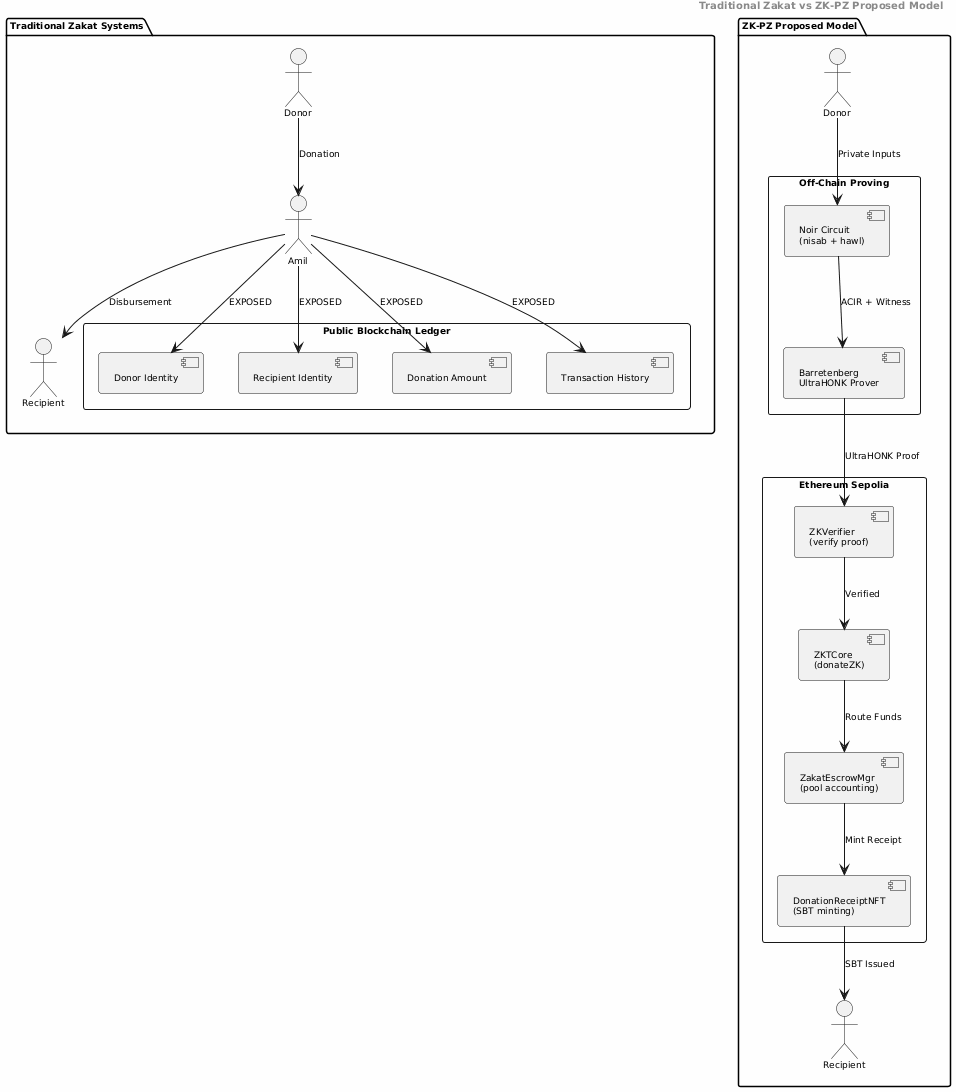
\includegraphics[width=0.92\columnwidth]{background_model.png}
\caption{Traditional Zakat Paradigm vs. Proposed ZK-PZ Model}
\label{fig:background}
\end{figure}

\section{Research Methodology}

This study adopts a Design Science Research (DSR) approach, summarized in Fig.~\ref{fig:dsr}.

\begin{figure}[!ht]
\centering
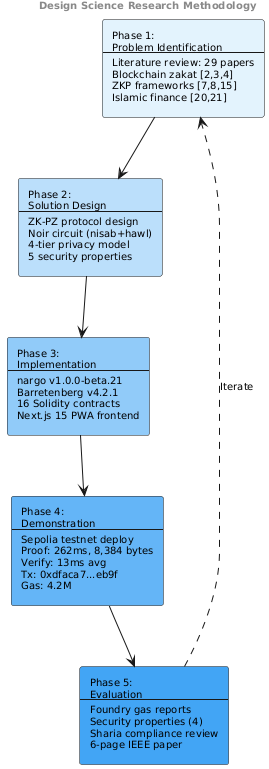
\includegraphics[width=0.48\columnwidth]{research_methodology.png}
\caption{Design Science Research Methodology: five phases from problem identification to evaluation}
\label{fig:dsr}
\end{figure}

\section{Proposed ZK Private Zakat Protocol}

\subsection{System Overview and Threat Model}

The ZK-PZ protocol operates within a five-actor trust model: donor (ZKP prover and private note creator), recipient (private note receiver), amil institution (verifier and eligibility attestor), Aztec Network (private transaction infrastructure), and Ethereum Sepolia (public settlement layer).

The threat model assumes: (1)~an honest-but-curious verifier, (2)~a potentially malicious claimant, and (3)~a public blockchain network subject to transaction graph analysis. The protocol guarantees the properties summarized in Table~\ref{tab:properties}.

\begin{table}[htbp]
\caption{ZK-PZ Protocol Security Properties}
\label{tab:properties}
\small
\begin{center}
\begin{tabular}{|p{1.7cm}|p{6.6cm}|}
\hline
\multicolumn{1}{|c|}{\textbf{Property}} & \multicolumn{1}{c|}{\textbf{Guarantee}} \\
\hline
Donor anonymity & Identities, amounts, and patterns never exposed on-chain; only ZK proofs of valid donation are publicly verifiable. \\
\hline
Recipient privacy & Zakat disbursed through encrypted private notes; eligibility verified without attribute disclosure. \\
\hline
Soundness & Non-eligible recipient cannot generate an accepted proof under q-PKE assumption \cite{b_zkp_blockchain}. \\
\hline
Double-donation & Nullifier hash prevents the same recipient from claiming zakat more than once per cycle. \\
\hline
Institutional accountability & Amil institutions verify aggregate compliance without accessing individual transaction data \cite{b_maqasid_data,b_maqasid_privacy}. \\
\hline
\end{tabular}
\end{center}
\end{table}

\subsection{System Architecture and Payment Flow}

The platform employs a hybrid architecture combining Noir circuits on the client side with Ethereum Sepolia for public settlement. Donors pay in stablecoins or ETH; funds flow through off-chain proof generation and on-chain verification via the \texttt{donateZK()} function. This design ensures that individual donation privacy is maintained through cryptographic proofs while institutional accountability is achieved through on-chain event emission and nullifier tracking.

A Progressive Web Application supports the donor-facing workflow, providing wallet connection, privacy tier selection, donation amount input, proof generation visualization, and transaction confirmation. Proof generation runs in a Web Worker ensuring that private inputs never leave the donor's device \cite{b_zkp_blockchain}.

\section{Evaluation}

Circuit benchmarks used Noir v1.0.0-beta.21 and Barretenberg v4.2.1. Gas measurements from Foundry on a local Sepolia fork.

\subsection{Circuit Performance}

\begin{table}[htbp]
\caption{ZakatEligibility Circuit Performance: UltraHONK evm target, $n=5$ runs}
\label{tab:proof_perf}
\begin{center}
\begin{tabular}{|l|r|}
\hline
\multicolumn{1}{|c|}{\textbf{Metric}} & \multicolumn{1}{c|}{\textbf{Value}} \\
\hline
ACIR opcodes               & 29 \\
Brillig opcodes            & 44 \\
Proof generation (avg)     & 261.8 ms \\
Proof verification (avg)    & 13.0 ms \\
Proof size                  & 8,384 bytes \\
\hline
\end{tabular}
\end{center}
\end{table}

\subsection{Sepolia Deployment and Gas Consumption}

Sixteen contracts were deployed to Sepolia (chain ID 11155111). The ZKTCore (v5) routes \texttt{donateZK()} through \texttt{zakatEscrowManager.donate()} for pool accounting. An end-to-end donation (tx 0xdfaca7...eb9f) completed verification, nullifier registration, transfer, NFT minting, and event emission in 4.2\,M gas.

Table~\ref{tab:gas} reports gas costs measured via Foundry gas reports.

\begin{table}[htbp]
\caption{Smart Contract Gas Consumption: Foundry Gas Report, Sepolia Fork}
\label{tab:gas}
\small
\begin{center}
\begin{tabular}{|l|l|r|}
\hline
\textbf{Contract} & \textbf{Function} & \textbf{Gas (avg)} \\
\hline
ZKTCore               & \texttt{donate()}                   & 490,187 \\
ZKTCore               & \texttt{createCampaignPool()}       & 365,552 \\
ZKTCore               & \texttt{castVote()}                 & 132,909 \\
ZKTCore               & \texttt{donateZK()} (e2e)            & 4,200,000 \\
\hline
ZKTCore               & Deploy                              & 5,314,471 \\
ZakatEscrowManager    & Deploy                              & 3,069,194 \\
ShariaReviewManager   & Deploy                              & 2,114,307 \\
\hline
\end{tabular}
\end{center}
\end{table}

\subsection{Security Analysis}

\textbf{Donor anonymity}: Donor identities and amounts are never exposed on-chain; only ZK proofs are publicly verifiable \cite{b_aztec,b_zkp_cacm}. \textbf{Recipient privacy}: Zakat is disbursed through encrypted notes with eligibility verified without attribute disclosure \cite{b_bbs_w3c}. \textbf{Circuit soundness}: Under the q-PKE assumption \cite{b_zkp_blockchain}, forging a proof is computationally infeasible \cite{b_zkp_vuln}. \textbf{Double-donation prevention}: The Pedersen nullifier binds each claim to a unique donor and cycle, with atomic rejection of duplicate claims \cite{b_zkp_idm}.

\section{Discussion}

\subsection{Sharia Compliance and Deployment}

The protocol aligns with maqasid al-shariah \cite{b_maqasid_data,b_maqasid_privacy,b_maqasid_blockchain}: \textit{nafs} (dignity) protection ensures donor/recipient financial privacy; \textit{mal} (wealth) uses cryptographic integrity; \textit{amanah} (trustworthiness) via on-chain verification \cite{b_zakat_transparency}. Deployment requires Aztec integration, amil training, and OJK Sandbox alignment.

\subsection{Limitations and Future Work}

Circuit scope is limited to nisab and hawl criteria; the architecture accommodates all eight asnaf categories. Future work includes recursive proof systems, extension to additional asnaf categories, compliance-friendly ZK protocols, and batched settlement optimization \cite{b_zkp_circuits,b_zkfi,b_halal_crypto}.

\section{Conclusion}

This paper presented a Zero-Knowledge Private Zakat (ZK-PZ) protocol addressing the privacy paradox in blockchain-based zakat systems. An implementation using Noir circuits (29 ACIR opcodes) with UltraHONK proving via Barretenberg v4.2.1 was deployed to Ethereum Sepolia, achieving proof generation in 262\,ms and end-to-end donation in 4.2\,M gas. The work reconciles cryptographic privacy with \textit{nafs} preservation in Islamic social finance \cite{b_maqasid_data, b_maqasid_privacy}, demonstrating that institutional accountability and individual privacy are simultaneously achievable through applied cryptography.

\section*{Acknowledgment}

This research was conducted as part of a hackathon project at BINUS University. The authors thank the Ethereum Jakarta community for technical support and Tawf Labs teammates for sharia consultation. The codebase is available at \url{https://github.com/tawf-labs/zkt-hackathon} and the testnet at \url{https://ziswaf.tawf.foundation}. The authors acknowledge the use of AI-assisted tools for code scaffolding and formatting. Core algorithmic contributions and protocol design were developed by the authors.

\begin{thebibliography}{00}

\bibitem{b_baznas}
BAZNAS, ``Outlook Zakat Indonesia 2022,'' Badan Amil Zakat Nasional, Jakarta, Indonesia, 2022. [Online]. Available: \url{https://baznas.go.id}

\bibitem{b_zakat_acm}
H. Babas et al., ``A blockchain based decentralized zakat collection and distribution platform,'' in \textit{Proc. ACM Int. Conf.}, 2024, doi:~10.1145/3641067.3641071.

\bibitem{b_zakat_malaysia}
A. Nazeri et al., ``Exploration of a new zakat management system empowered by blockchain technology in Malaysia,'' \textit{ISRA Int. J. Islamic Finance}, 2023, doi:~10.55188/ijif.v15i4.568.

\bibitem{b_zakat_transparency}
M. Khairi et al., ``The development and application of the zakat collection blockchain system,'' \textit{Virtus Interpress}, 2023, doi:~10.22495/jgrv12i2siart12.

\bibitem{b_maqasid_data}
``Maqasid al-Shariah and the digital data ownership,'' \textit{J. Islamic Law Digit. Econ. Bus.}, vol.~1, no.~2, pp.~168--181, 2022. [Online]. Available: \url{https://journal.uii.ac.id/JILDEB/article/view/46815}

\bibitem{b_maqasid_privacy}
``Sharia governance and personal data protection in Islamic fintech,'' \textit{Hukmuna}, 2022. [Online]. Available: \url{https://journals.ai-mrc.com/hukmuna/article/view/913}

\bibitem{b_zkp_circuits}
J. Wen et al., ``Practical security analysis of zero-knowledge proof circuits,'' in \textit{Proc. 33rd USENIX Security Symp.}, 2024, ISBN 978-1-939133-44-2. [Online]. Available: \url{https://www.usenix.org/conference/usenixsecurity24/presentation/wen}

\bibitem{b_zakat_biblio}
M. Fauzi, P. Paiman, and O. Othman, ``A bibliometric analysis of blockchain-based zakat system design,'' \textit{Acad. J. Interdiscip. Stud.}, vol.~14, no.~1, 2025. [Online]. Available: \url{https://www.richtmann.org/journal/index.php/ajis/article/view/13846}

\bibitem{b_zkp_financial}
O. V. Kovalchuk and M. P. Karpiak, ``Zero-knowledge proof framework for privacy-preserving financial transactions,'' \textit{Sci. Bull. Lviv Polytech. Nat. Univ.}, no.~1(151), pp.~129--136, 2024. [Online]. Available: \url{https://science.lpnu.ua/sdil/vsi-vypusky/volume-10-number-1-151-2024}

\bibitem{b_ziswaf_blockchain}
I. M. Unal and A. F. Aysan, ``FinTech, digitalization, and blockchain in Islamic finance: Retrospective investigation,'' \textit{FinTech}, vol.~1, no.~4, pp.~388--398, 2022, doi:~10.3390/fintech1040029.

\bibitem{b_zkp_blockchain}
A. Hameed, A. Farooq, and M. Usman, ``Zero knowledge proofs: A comprehensive review of applications, protocols, and future directions in cybersecurity,'' \textit{IEEE Access}, vol.~11, pp.~87429--87449, 2023, doi:~10.1109/ACCESS.2023.3297314.

\bibitem{b_aztec}
Aztec Network, ``Aztec's ZK-ZK-Rollup: Looking behind the cryptourtain,'' \textit{Aztec Blog}, 2022. [Online]. Available: \url{https://aztec.network/blog/aztecs-zk-zk-rollup-looking-behind-the-cryptocurtain}

\bibitem{b_noir}
Noir Language, ``Noir Documentation,'' 2024. [Online]. Available: \url{https://noir-lang.org/docs/}

\bibitem{b_poseidon}
L. Grassi, D. Khovratovich, C. Rechberger, A. Roy, and M. Schofnegger, ``Poseidon: A new hash function for zero-knowledge proof systems,'' in \textit{Proc. 30th USENIX Security Symp.}, pp.~519--535, 2021, ISBN 978-1-939133-24-4.

\bibitem{b_aztec_nr}
Aztec Network, ``Introducing Aztec.nr: Aztec's Private Smart Contract Framework,'' \textit{Aztec Blog}, Sep. 2023. [Online]. Available: \url{https://aztec.network/blog/introducing-aztec-nr}

\bibitem{b_bbs_w3c}
S. Tessaro and C. Zhu, ``Revisiting BBS Signatures,'' in \textit{Advances in Cryptology -- EUROCRYPT 2023}, ser. LNCS, vol.~14008, Springer, 2023, pp.~691--721, doi:~10.1007/978-3-031-30589-4\_24.

\bibitem{b_mixer_analysis}
Z. Wang, S. Chaliasos, K. Qin, L. Zhou, L. Gao, P. Berrang, B. Livshits, and A. Gervais, ``On How Zero-Knowledge Proof Blockchain Mixers Improve, and Worsen User Privacy,'' in \textit{Proc. ACM Web Conf. 2023 (WWW '23)}, 2023, pp.~2022--2032, doi:~10.1145/3543507.3583217.

\bibitem{b_zkfi}
V. Buterin, J. Illum, M. Nadler, F. Sch\"{a}r, and A. Soleimani, ``Blockchain privacy and regulatory compliance: Towards a practical equilibrium,'' \textit{Blockchain: Res. Appl.}, vol.~5, no.~1, Art. no.~100176, Mar. 2024, doi:~10.1016/j.bcra.2023.100176.

\bibitem{b_zkp_idm}
A. M\"{u}hle, K. Assaf, and C. Meinel, ``One to bind them: Binding verifiable credentials to user attributes,'' in \textit{Proc. SECRYPT}, 2023, doi:~10.5220/0012057900003555.

\bibitem{b_isf_covid}
I. S. Beik and L. S. Arsyianti, ``The role of Islamic social finance during Covid-19 pandemic in Indonesia's economic recovery,'' \textit{Int. J. Islamic Middle Eastern Finance Manage.}, vol.~14, no.~4, pp.~704--720, 2021, doi:~10.1108/IMEFM-01-2021-0028.

\bibitem{b_zakat_emerald}
A. H. Mohd et al., ``Blockchain technology in zakat management: potential and challenges,'' \textit{J. Islamic Account. Bus. Res.}, vol.~15, no.~3, pp.~567--583, 2024, doi:~10.1108/JIABR-08-2022-0206.

\bibitem{b_zkp_cacm}
A. Williams, ``Zero-knowledge proofs and their role within the blockchain,'' \textit{Commun. ACM}, vol.~67, no.~7, pp.~78--87, Jul. 2024, doi:~10.1145/3663705.

\bibitem{b_maqasid_blockchain}
M. N. A. Aziz and N. M. Salleh, ``Innovation in Islamic finance: Integrating blockchain with Maq\={a}\d{s}id al Shar\={\i}`ah and \d{H}if\d{z} al M\={a}l,'' \textit{J. Emerg. Econ. Islamic Res.}, vol.~13, no.~1, 2025, doi:~10.24191/jeeir.v13i1.3852.

\bibitem{b_halal_crypto}
A. R. Ibrahim and M. Y. Zulkifli, ``Toward an Islamic cryptocurrency: A proposed halal coin,'' \textit{J. Account. Finance}, vol.~25, no.~3, pp.~64--78, 2025, doi:~10.33423/jaf.v25i3.7858.

\bibitem{b_hybrid_zk}
M. A. Mohamed, A. Hassan, and K. Elsayed, ``Hybrid zk-STARK and zk-SNARK framework for privacy-preserving smart contract data feeds,'' in \textit{Proc. IEEE ICCA}, 2024, doi:~10.1109/ICCA62237.2024.10928100.

\bibitem{b_zkp_vuln}
N. Ivanov, C. Li, and Q. Yan, ``Zero-knowledge proof vulnerability analysis and security auditing,'' \textit{Cryptology ePrint Archive}, Rep. 2024/514, 2024. [Online]. Available: \url{https://eprint.iacr.org/2024/514}

\bibitem{b_rbac_sc}
J. P. Cruz, Y. Kaji, and N. Yanai, ``RBAC-SC: Role-based access control using smart contract,'' \textit{IEEE Access}, vol.~6, pp.~12240--12251, 2018, doi:~10.1109/ACCESS.2018.2812844.

\bibitem{b_pwa_survey}
S. Khan and M. Ahmad, ``A survey on progressive web applications for decentralized systems,'' \textit{Preprints}, 2024, doi:~10.20944/preprints202403.0891.v1.

\bibitem{b_nft_review}
M. Wang, Q. Li, and Z. Zheng, ``Beyond collectibles: A comprehensive review of non-fungible token applications,'' \textit{IEEE Trans. Serv. Comput.}, vol.~16, no.~6, pp.~4184--4200, 2023, doi:~10.1109/TSC.2023.3310823.

\end{thebibliography}

\end{document}
